\documentclass{VUMIFPSkursinis}
\usepackage{algorithmicx}
\usepackage{algorithm}
\usepackage{algpseudocode}
\usepackage{amsfonts}
\usepackage{amsmath}
\usepackage{bm}
\usepackage{caption}
\usepackage{color}
\usepackage{float}
\usepackage{graphicx}
\usepackage{listings}
\usepackage{subfig}
\usepackage{wrapfig}
\usepackage{url}

% Titulinio aprašas
\university{Vilniaus universitetas}
\faculty{Informatikos fakultetas}
\department{Programų sistemų katedra}
\papertype{Kursinis darbas}
\title{Asinchroninis sesijų komunikavimas Haproxy paskirstymo serveryje, taip padedant greičiau aptikti klaidas}
\titleineng{...}
\status{3 kurso 6 grupės studentas}
\author{Andrius Butkevičius}
% \secondauthor{Vardonis Pavardonis}   % Pridėti antrą autorių
\supervisor{doc. Karolis Petrauskas}
\date{Vilnius – \the\year}

% Nustatymai
% \setmainfont{Palemonas}   % Pakeisti teksto šriftą į Palemonas (turi būti įdiegtas sistemoje)
\bibliography{bibliografija}

\begin{document}
\maketitle

\tableofcontents

\sectionnonum{Įvadas}
	Didėjant žmonių kompiuteriniam raštingumui, interneto populiarumui, nesudėtinga pastebėti, kad atsiranda vis daugiau programinių ar internetinių aplikacijų, kurios vienaip ar kitaip palengvina darbuotojų užduotis, automatizuojant procesus(sumažinant rankinį darbą ir leidžiant paskirti laiką sudėtingesnioms užduotims) ar vykdant sudėtingas operacijas, kurios reikalauja įvairių integracijų: banko sąskaitos pervedimas, mokesčių mokėjimas.

	Nenorint, kad vartotojai ar kitos sistemos, kurios naudojasi kurtomis integracijomis, susidurtų su problemomis, kurių metu nebūtų galima efektyviai naudotis sistema ar ją iš vis pasiekti be nesklandumų, kai ji yra apkrauta didelu prisijungusių vartotojų kiekiu. Todėl vis daugiau programavimo įmonių skiria dėmesį sistemos serverių architektūrai, pasitelkiant nebe monolitinius serverius, o jų šeimas, taip darbo krūvį paskirstant keliems išoriniams serveriams ir taip išvengiant apkrovos ar problemų su pralaidumu.

	Visgi apsisaugoti nuo serverio ryšio problemų, tokių kaip nutrūkęs serverio ryšys neįmanoma, todėl reikia ieškoti sprendimo būdų, kurie kuo įmanoma labiau sumažintų patiriamos klaidos pasėkmes klientui, leidžiant tas klaidas užfiksuoti kuo greičiau, ir taip suvaldant situaciją išanksto.

	Šiame kursiniame darbe bus nagrinėjamas algoritmas ir įgyvendinamas į vieną populiariausių atviro kodo paskirstymo serverių-  „HaProxy" [www.haproxy.org]. Apžvelgsiu kaip šis algoritmas susitvarko su nutrūkusiu ryšių tarp kelių sistemų, palyginsiu jį su kitais sprendimo būdais naudojamais šiomis dienomis.

	Algoritmas sprendžia problemą, kaip greičiau ir su mažiau nepageidaujamų pašalinių pasėkmių informuoti klientą apie įvykusią klaidą. Algoritmo veikimo principas naudoja sesijų valdymą, kurios tarpusavyje komunikuoja asinchroninėmis žinutėms tais atvejais, kai ištinka serverio vidinė klaida ir vienas iš serverių tampa nebepasiekiamas vartotojui. Tokiu atveju įgyvendintantas algoritmas nedelsiant praneštų apie nutrukūsį ryši su serveriu ir perspetų esančias klientų sesijas.

	 Šio darbo tikslas yra įgyvendinti aprašyta algoritmą Haproxy paskirstymo serveryje, paieškoti alternatyvių sprendimo būdų, juos palyginti, ištirti kaip tai veikia kartu su kitais rinkoje naudojamais sprendimo būdais, tokiais kaip „Round Robin“, „Leastconn“.

\section{Load balancing}
Kompiuterių sistemų terminologijoje „Load balancing“ reiškia mechanizmą, kuris leidžia pagerinti ir paefektyvinti darbo krūvio paskirstymą tarp skaičiavimus gebenačių sistemų, kai yra nauojami "application clusters" - aibė kompiuterių, kurie tarpusavyje veikia kartu, taip sukurdami viena kompiuterių šeimą, dėl kurios tai atrodo tarsi viena sistemą, o pati apkrova yra paskirstoma tolygiai, taip išvengiant bandwidth problemų.[https://link.springer.com/article/10.1007/s10586-018-2850-3]

Anksčiau vienas iš pagrindinių sprendimo būdų buvo DNS paskirstymas, naudojant Round-robin, kai svetainės vardui yra priskiriami keli ir daugiau IP adresų, kurie nurodo į skirtingus serverius. Visgi trūkumai, kad paskirstymas yra nenuspėjamas, susiduriama su podėlio problemomis bei automotiniu klaidų išvengimu.

Todėl buvo prieita prie tobulesnių ir geresnių būdų, išskaidant užklausas į serverį, nesusiduriant su problemomis aprašytomis prieš tai. Kai tinklo srautas atkeliauja iš vartotojo į serverių paskirstytoja, o vėliau į tikrus serverius ir galiausiai grįžta atgal pas klientą.

Kaip ir minėta anksčiau, „Load balancing“ paskirsto darbo krūvį paskirstymas tarp skiringų serverių operuojant tinklu paremtais įrenginiais. Taip pat pašalina serverį automatiškai, jeigu šis tampa pasyvus (neveikiantys), išskaido tinklo eismą į individualias užklausas ir nusprendžia, kuris serveris gaus individualią užklausą.[Bourke 10 4psl]


\graphicspath{ {./img/} }
 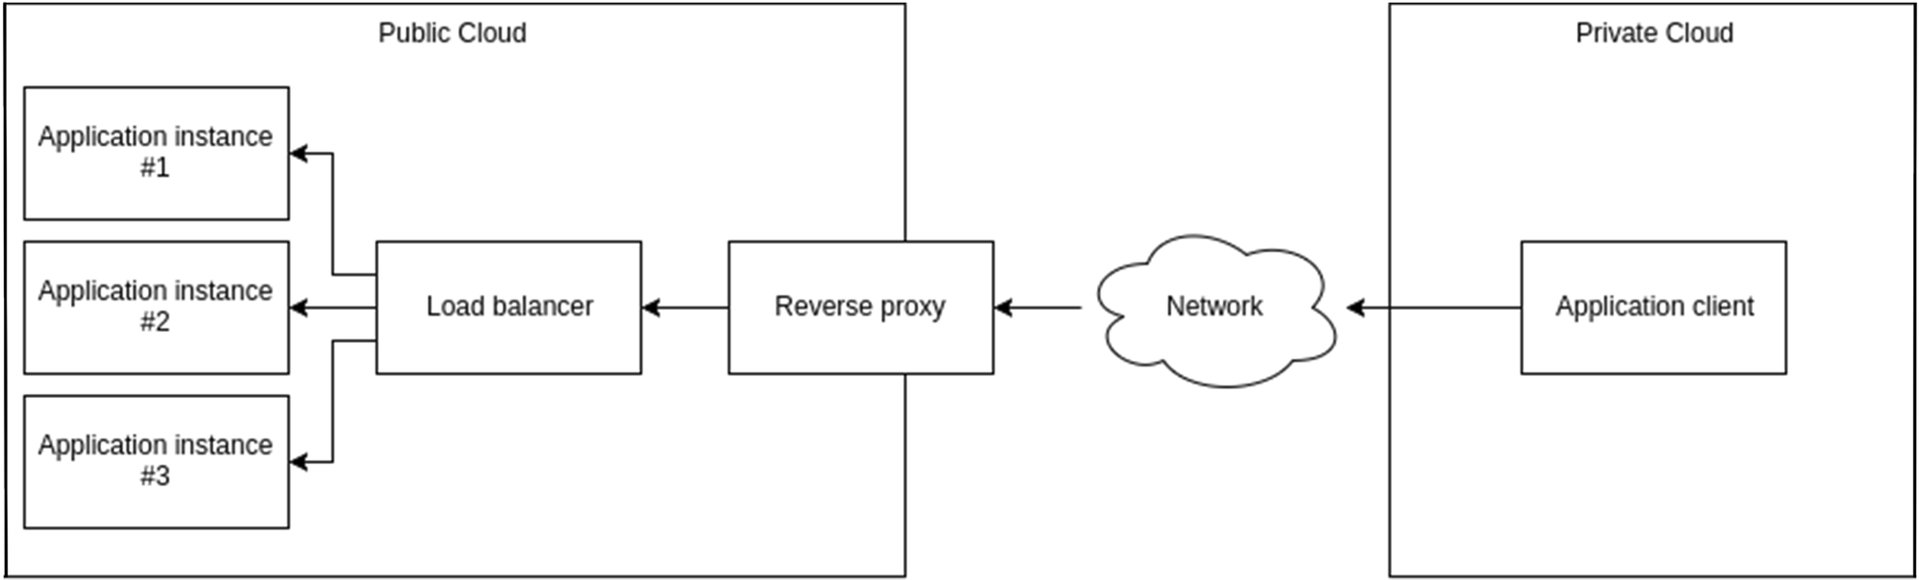
\includegraphics[width=150mm,scale=0.5]{load-balancing}

	Pačių algoritmų, paskirtančių darbą tarp serverių yra daug, o kurį būtent naudoti priklauso nuo esamos sistemos architektūros ir kokių poreikių jai reikia, nes krūvį galima paskirstyti tinklo(L4) ar aplikacijos sluoksnyje(L7). Pastarieji algoritmai skiriasi tuo, kaip jie geba stebėti ateinantį traffic ir pagal kokius kriterijus tą fiksuoja. Pavyzdžiui, L4 sugeba matyti informaciją apie aplikacijos portus, protokolo tipą (TCP/UDP), analizuojant keliaujančius paketus. Layer 7 „Load balancer“ mato detalesnę informaciją, todėl gali priimti ir paskirstyti „request“ naudojant sudėtingesnius sprendimų būdus. Su tokiu protokolu kaip HTTP įmanoma identitfikuoti kliento sesiją naudojant cookies, taip nukreipiant tam tikro vartotojo užklausas į tą patį serverį tol kol sesija yra nepasibaigusi, taip neprarandant informacijos, kuri yra saugoma tam tikrame serveryje. Taigi apibendrinant, aiškiausias skirtumas tarp jų toks, kad parenkamas serveris yra parenkamas L4 paskirstyme iškart kai yra gaunamas SYN paketas\cite{MsSyn} iš kliento, tuo metu L7 paskirstytojas parenka severį, kai tik jis gaus HTTP ar WebSocket žinutės užklausos paketą iš kliento.
 
Mano kursiniame darbe nagrinėsime Haproxy load balancing sistemą, kuri apdoroja užklausas, jau minėtame L7

\section{Klasterių serveriai}
	Čia išsiaiškinsime, ką reiškia šis terminas ir kuo tai yra susiję su mano nagrinėjama darbu. Klusterinimas reiškia skirstymas į aibes, grupes. Įgyvendinant programinę įrangą projekto metu turi būti atkreipiami nefunkciniai reikalavimai, tokie kaip maksimalus užklausų skaičius, kurį projektuojama sistema gebės apdoroti efektyviai, nesutrikdama ir išlaikydama greita procesų veikimą esant dideliam užklausų skaičiui. Visgi projektui plečiantis ir užklausų kiekiui didėjant, turi atsirasti galingesnė ir našesnė sistema, gebanti apdoroti daugiau procesų vienu metu. Todėl reikia projekto pradžioje apsvarstyti arhcitektūra, kuri būtų lengvai plečiama. Vieni iš būdų: "Scale-up" ir "Scale-out".

"Scale-up" reiškia, kad programinė įranga lienka prie monolitinės serverio architektūros, kurioje yra tik vienas serveris, ir kiekvieną kartą, kai reikės sistemą plėsti, bus paleidžiamas naujas serveris, gebantis daugiau procesų apdoroti.
\url {https://link.springer.com/article/10.1007/s10586-018-2850-3}

"Scale-out", kai sistemos architektūra susidaro ne iš vieno serverio, o iš kelių ir daugiau tinklo serverių, kurie sudaro viena bendrą serverių klasterį. Toks sprendimo būdas yra pigesnis, efektyvesnis, nes vos tik prireikus pajegesnės sistemos, pastarajai sistemai galima prijungti papildomą naują serverį. Taigi serverių šeimos yra vadinamos Clustered application ir norint jas suvaldyti reikalinga prieš ją stovinti programinė įranga(reverse proxy), kuri galėtų paskirstyti darbą tarp serverių po lygiai.

\section{Serverių paskirstymo būdai bei programinė įranga}
Kanangi dauguma programinės įrangos įmonių projektuoja tinklo serverius, dažniausiai paremtais HTTP ar WebSocket protokolas, bendraujant su klientu, komponentas atsakingas už įeinantį traffic yra paskirstymo serveris (pvz.: Haproxy) negu Edge router ar L4 (Transport Layer of OSI model) load balance, nes reverse-proxy siūlo daugiau galimybiu stebint traffic su HTTP protokolu, kaip pavyzdžiui load-balacing ar turinio glaudinimas.

Taip pat yra įmanomas kliento pusėje esantis krūvio paskirstymas, tačiau tai reikalauja atrandamumo(discoverability) ir prisijungiamumas (connectivity) savybių. Atrandamumas pasako būdą, kaip bus identifikuojama topologija - dažniausiai, skaičius serverių, nurodomų portų numerių bei IP adresų. Tokios informacijos užtenka klientui sukonfiguruoti reikiama aplikacijos baseiną(pool). Prisijungiamumas parodo kliento gebėjimą tiesiogiai prisijungti prie tų serverių.
Plačiausiai šiuo metu rinkoje yra paplitę paskirstytojai: „Haproxy“, „Ngnix“, „F5“, „Citrix ADC“, „Avi Vantage“, „AWS“. Skirtumai tarp šių paskirstytojų yra efekytvumas, našumas, naudojamai skirtingi algoritmai, stebėjimo sistemomis. Be to, jeigu nenorima patiems dėliotis techninės įrangos patiems, galima rinktis „cloud based solutions“, pavyzdžiui, „AWS“. Jeigu norima, kad sistema būtų kontroliuojama pačių programuotojų, reikia rinktis iš „Haproxy“, „Ngnix“/[https://www.techrepublic.com/article/data-center-101-choosing-a-load-balancer]

\subsubsubsection{Sesijos valdymas klasterinėje aplikacijoje}
Klasterių sistemai reikalingas patikimas ir efektyvus HTTP sesijų valdymas. Visgi perkeliant programinę įrangą į tokią aplinką yra susiduriama su keletą sunkumų. HTTP sesija apima nuoseklę kliento sąveiką su tinklo servisu. Ši sesijos būsena išlaikoma yra tam tikrą fiksuotą laiką. Kiekvieną kliento sesija yra priskiriama tam tikram serveriui. Taigi keletas serverių negali turėti vienos bendros sesijos konkečiam klientui, ar bent jau nėra įprasta, nes sesija yra laikoma individualiai serverio atmintyje ir keli serveriai tarpusavyje nesidalina šios informacijos. Kadangi HTTP protokolas neišlaiko būsenos(stateless), iš užklausos negalime nustatyti kokiam vartotojui ji priskiriama, todėl yra naudojama sesija, kad būtų talpinama tokia informaciją, tačiau klasterinėse sistemose, jeigu yra svarbu, kad klientas išlaikytų sesiją su tuo pačiu serveriu, reikia užtikrinti, kad klientas visada galėtų pasiektį būtent tą severį, su kuriuo buvo pradėta sesija. Į pagalbą ateina „Sticky sessions“, kurioje yra laikomas IP adresas serverio į kūrį buvo iš pradžių kreiptasi, vėliau „Load balancer“ pagal tai kokia yra informacija sesijos, nukreips užklausą į tinkamą serverį. Kitas pavyzdys su kuriuo yra susiduriama, kai sistema turi kelis serverius, tačiau nėra implementavę sticky sessions, kad keli serveriai turi atskirus „pool“, kuriuose yra laikoma aplikacijos informaciją, pavyzdžiui – jeigu ASP.NET sistemoje pasirinksime inicializuoti objektą „web“ aplikacijoje kaip Singleton, sukurti objektai tam serveryje bus pasiekiami tik iš to serverio, todėl jei užklauso nukreipia į kitą serverį mes prarandame dabartinę OOP terminais kalbant, objekto esamą informaciją, kurios negalime pasiekti tol, kol užklausa vėl nebus nukreipta į reikiamą serverį.

\section{Event-driven arhcitektūra}
Šio kursinio darbo algoritme, svarbią dalį užema asinchroninis komunikavimas, kuris neretai dar yra įvardijamas kaip event-based komunikavimas.
Įvykiais paremtra architektūra sugeba aptikti įvykstančius įvykius ir į juos atsakyti protingai. \url{https://books.google.lt/books?hl=lt&lr=&id=g1318W0CIm4C&oi=fnd&pg=PT8&dq=event+driven+architecture&ots=Vrqbe8Sdi_&sig=FKh3XUNF9YwanbpiVqIusUqKfDo&redir_esc=y#v=onepage&q=event%20driven%20architecture&f=false}

Įvykis - pokytis būsenos, kuris yra svarbus vidinėms ir išorinėms sistemoms. Norint pasiekti tokią architektūrą, reikia ją sumodeliuoti taip, kad joje atsispindėtų procesai, kaip aptikti įvykius, perduoti žinutes tarp komponentų, tarp kurių įvykis įvyko, jį perduoti kitai sistemai, taip informuojant apie jai svarbų įvykį, kad tokiu būdų komponentas galėtų reaguoti pagal jo paskirtį. Bendriniai terminai šiuos gebėjimus įvardijant yra event-producer, event-consumer, massing-backbones bei event processors
Kitas terminas, kūrį perskaitome kursinio darbo pavadinimė – asinchroninis komunikavimmas. 
\section{HaProxy}
Tai vienas populiariausių rinkoje “open source” serverių paskirstytojų, parašytų C kalba, kuri padeda užtikrinti efektyvų ir našų veikimą. “Load-balancer” serveriai dar taip pat yra žinomi, kaip “front-end” serveriai. Kiekvienas iš serverių turi skirting IP adresą, tačiau dalinasi tuo pačiu “domain address”. “HaProxy” taip pat yra nemokamas, labia greitas ir puikus sprendimas naudojant kartu su HTTP ar TCP protokolais paremtais servisais. Kadangi tai “open source”, tai šis “load-balancer” turi puikiai palaikomas programuotojų, ir jau per laiką, kurį jis yra išleistas, buvo nemažai naujų versijų, kurioje yra papildoma naujom galimybėm. Šiuo metu  naujausia versija yra 1.8 (palaikomas “multi-threading”, HTTP/2, “cache” ir t.t). Vartotojui taip pat atsiveria galimybė šį “Load-balancer” konfiguruoti ir pritaikyti pagal savo poreikius – reguliuoti kokius port’us turės “front-end” ir “back-end” serveriai, koks bus “session-stickness” gyvavimo laikotarpis, “logging”, maksimalus kiekis užklausų, nurodyti kiekį turimų gijų ir procesų, “timeout connect” laukimo trukmės laikotarpis, kokie port’ai yra “front-end” serveriuose(į juos kreipsis klientai pirma, vėliau užklausos bus paskirstytos į “back-end” serverius, koks bus naudojamas paskirstymo algoritmas.

“HaProxy” palaikomi paskirstymo tarp serverių algoritmai, kaip ir minėjau iš anksčiau yra konfiguruojami “haproxy.cfg” konfiguracijos globaliame faile.

Round-Robin – paskirsto užklausas nuosekliai, neatsižvelgiant kokia yra serverių dabartinė talpa ar apkrova. Visi serveriai yra laikomi vienaverčiais

Least-connection – paskirstomos užklausos pagal tai, kaip kiekvienas serveris yra aktyvus (apkrautas), serveris, kuriam šiuo metu tenka mažiau apdoroti užklausų gaus būtent ką tik atėjusią užklausą.

\section{Algoritmas}
Mano nagrinėjamas kursinis darbas peržvelgia algoritmą, kuris sprendžia problemą, kai vienas iš provider serverių tampa neatktyvus, nors tuo metu buvo inicializavęs ryšį su klientu, tačiau klientas negali apie tai sužinoti tol kol nesikreips į tą serverį arba baigsis time-out ryšio. 

Realiuose gyvenimo pavyzdžiuose nutinka taip, kad kartais vienas iš severių atsijungia dėl įvarių priežasčių, kaip kad nebuvo atlaikytas užklausų skaičius. Taigi turime situacija, kai netenkama vieno iš serverių, jeigu klientas tuo metu turėjo aktyvų ryšį, jo nebelienka, visgi kad klientas gautų informaciją apie tai, kad ryšys nutrūko prireikia laiko, nes praradus “connection” nebėra įmanoma pranešti tai vartotojams, nenaudojant jokių mofikacijų. Taigi galiausiai klientas gaus “timout connection error”, kuris ir reiškia, kad išorinė sistema nebeatsako po jai duoto maksimalaus laiko. Tačiau tai nėra geriausias sprendimas, jis yra lėtas aptinkant klaidas. Mano nagrinėjamame algoritme yra aprašomas būdas, kaip to išvengti implementuojant “fault-tolarant” algoritmą.
 
Sesijų valdymo algoritmas informuoja “client-side” (HaProxy front-end node’as) sesijos koordinatorių apie įvykusią klaidą “provider node”. Vėliau koordinatorius informuoja kitas sesijas priskirtas prie to pačio back-end’o ir kitiems koordinatoriams esantiems kituose front-end mazguose. Tokiu atveju vartotojas gautų iš karto informuojančią klaidą apie sutrikusį serverio ryšį. Aišku tokiu atveju galima bandyti klientui sukurti naują sesiją kitame veikiančiame serveryje, tačiau naujas sesijos sukūrimas yra gana brangi operacija, reikalaujanti nemažai resursų bei atsiranda tikimybė dėl informacijos praradimo naujos sesijos metu. Mūsų atveju sesija nebūtų priskirta prie jokio serverio tol kol klientas vėl ne per  naujo prisijungs prie sistemos.

\graphicspath{ {./img/} }
 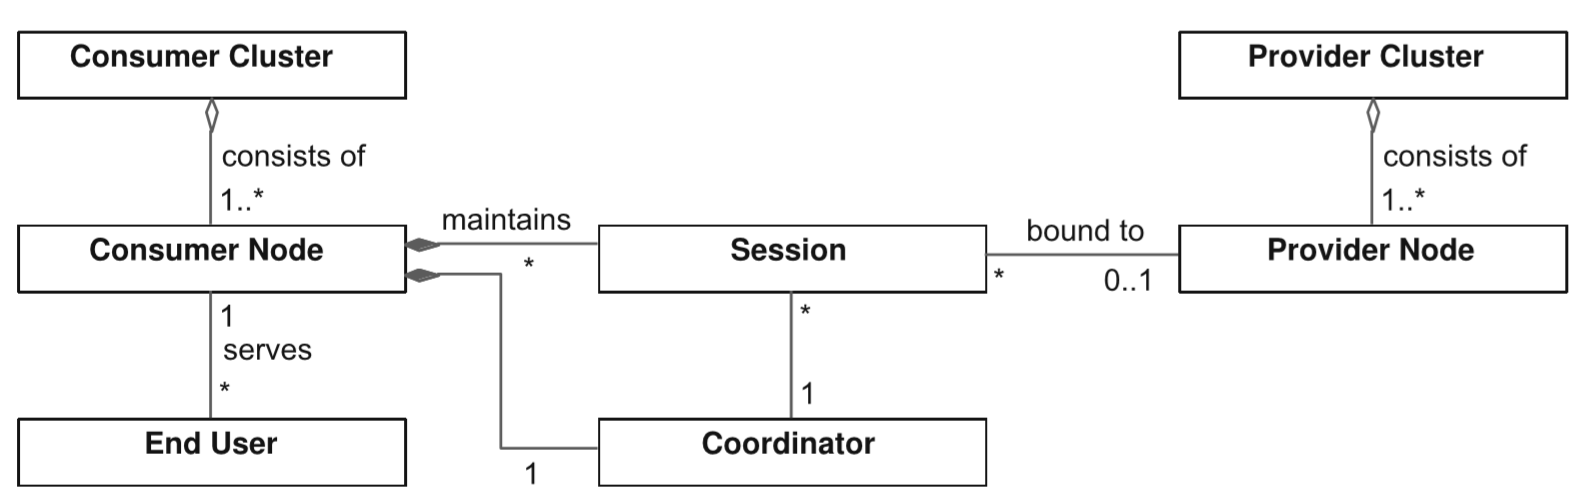
\includegraphics[width=150mm,scale=0.5]{structure}
\url {https://link.springer.com/chapter/10.1007/978-3-319-97571-9_11}

\section{Komunikavimo įgyvendinimas tarp sesijų}
Norint pasiekti, kad sesija galėtų komunikuoti su koordinatoriumi, o koordinatorius su kitais kliento koordinatoriais reikia pasitelkti asinchroninį programavimą.
Šiame skyrelyje aprašysiu, kaip veikia asinchroninis komunikavimas, kokie jo privalumai, kuo jis skiriasi nuo “event based” programavimo.

Asinchroninis perdavimas - duomenų perdavimo būdas, kai kiekvieno ženklo arba ženklų grupės perdavimo pradžios laikas neapibrėžtas, o nustatomas pagal specialius pradžios ir pabaigos bitus.
Tarpai tarp siunčiamų ženklų arba jų grupių gali būti nevienodi.

Tai ypač yra naudinga tarp web services, kai užklausos atsakymo laikas yra per daug ilgas ar sunkiai nuspėjamas, nėra norima apkrauti klientą laukiant atsako ir taip naudojant CPU.
\url{https://link.springer.com/chapter/10.1007/11581062_33}

Skirtumas tarp tarp šių dviejų paradigmų toks, kad “event driven” programavime objektas iškviečia “event” vos tik kai kažkas svarbaus įvyko, be jokių “polling” įgyvendinimo būdų, kai yra reguliariai žiūrima ar statusas pasikeitęs ar ne. Įvykus naujam statuso pasikeitmui programuotojas turi arba sinchroniškai, arba asinchroniškai užbaigti įvykusią operaciją.

Kai įvyksta asinchroninis operacija, sistema nelaukia, kada ši operacija bus įgyvendinta, todėl visa ši operacija yra įgyvendinama background’e, jos nelaukiant kada jis pasibaigs, visgi vos tik operacija atliekama, sistema, kuri ją kvietė gauna vadinama “call back” – pranešima, kad operacija daugiau nebėra vykdoma, ji arba įvyko, arba buvo susidurta su problemomis dėl kurios ji negalėjo sėkmingai finišuoti.

\sectionnonum{Šaltiniai}

\url{https://link.springer.com/article/10.1007/s10586-018-2850-3}

\url{https://link.springer.com/chapter/10.1007/11581062_33}

\url{https://link.springer.com/chapter/10.1007/978-3-319-97571-9_11}


\end{document}
